
To enhance the sensitivity to the Higgs boson signal, we apply additional 
$m_{\rm{H}}$ hypothesis dependent selections on the the following three variables:

%%%%%%%%%%%%%%%%%%%
\begin{enumerate}
\item $\met$,
\item Higgs transverse mass $M_{T}$ defined as,

\begin{equation}
M_{T}^{2} = \left( \sqrt{p_{T\mathrm{ ll}}^{2} + M_{ll}^{2}} + \sqrt{(\met)^{2} + M_{ll}^{2}} \right)^{2} - \left(\vec{p_{T\mathrm{ ll}}} + \vec{\met}\right)^{2}, \\
\label{eq:MTHZZ}
\end{equation}

\item $\Delta\phi$ between the $\met$ and the nearest jet if the jet $\Et > 30\ \GeV$, referred to as $\Delta\phi(jet,\met)$.
Expected distribution at the preselection level is shown in Figure \ref{fig:mtemloosesel}.
\end{enumerate}
%%%%%%%%%%%%%%%%%%%

The selection on the $\Delta\phi(jet,\met)$ is introduced to reduce the \dyll\ background, where the 
\met\, is mainly due to the jet mis-measurement. The optimization of the selections on the 
above three variables are described in Ref.~\cite{HZZ2011EPS}, with the lateset 
values shown in Ref.~\cite{hzzcutbase} and in Table \ref{tab:cut_selection}.
%Tables \ref{tab:HiggsSelectionCutBased} shows the expected 

%%%%%%%%%%%%%%%
\begin{figure}[!hbtp]
\begin{center}
\subfigure[$ee$]{\label{subfig:dphijetmet_ee}
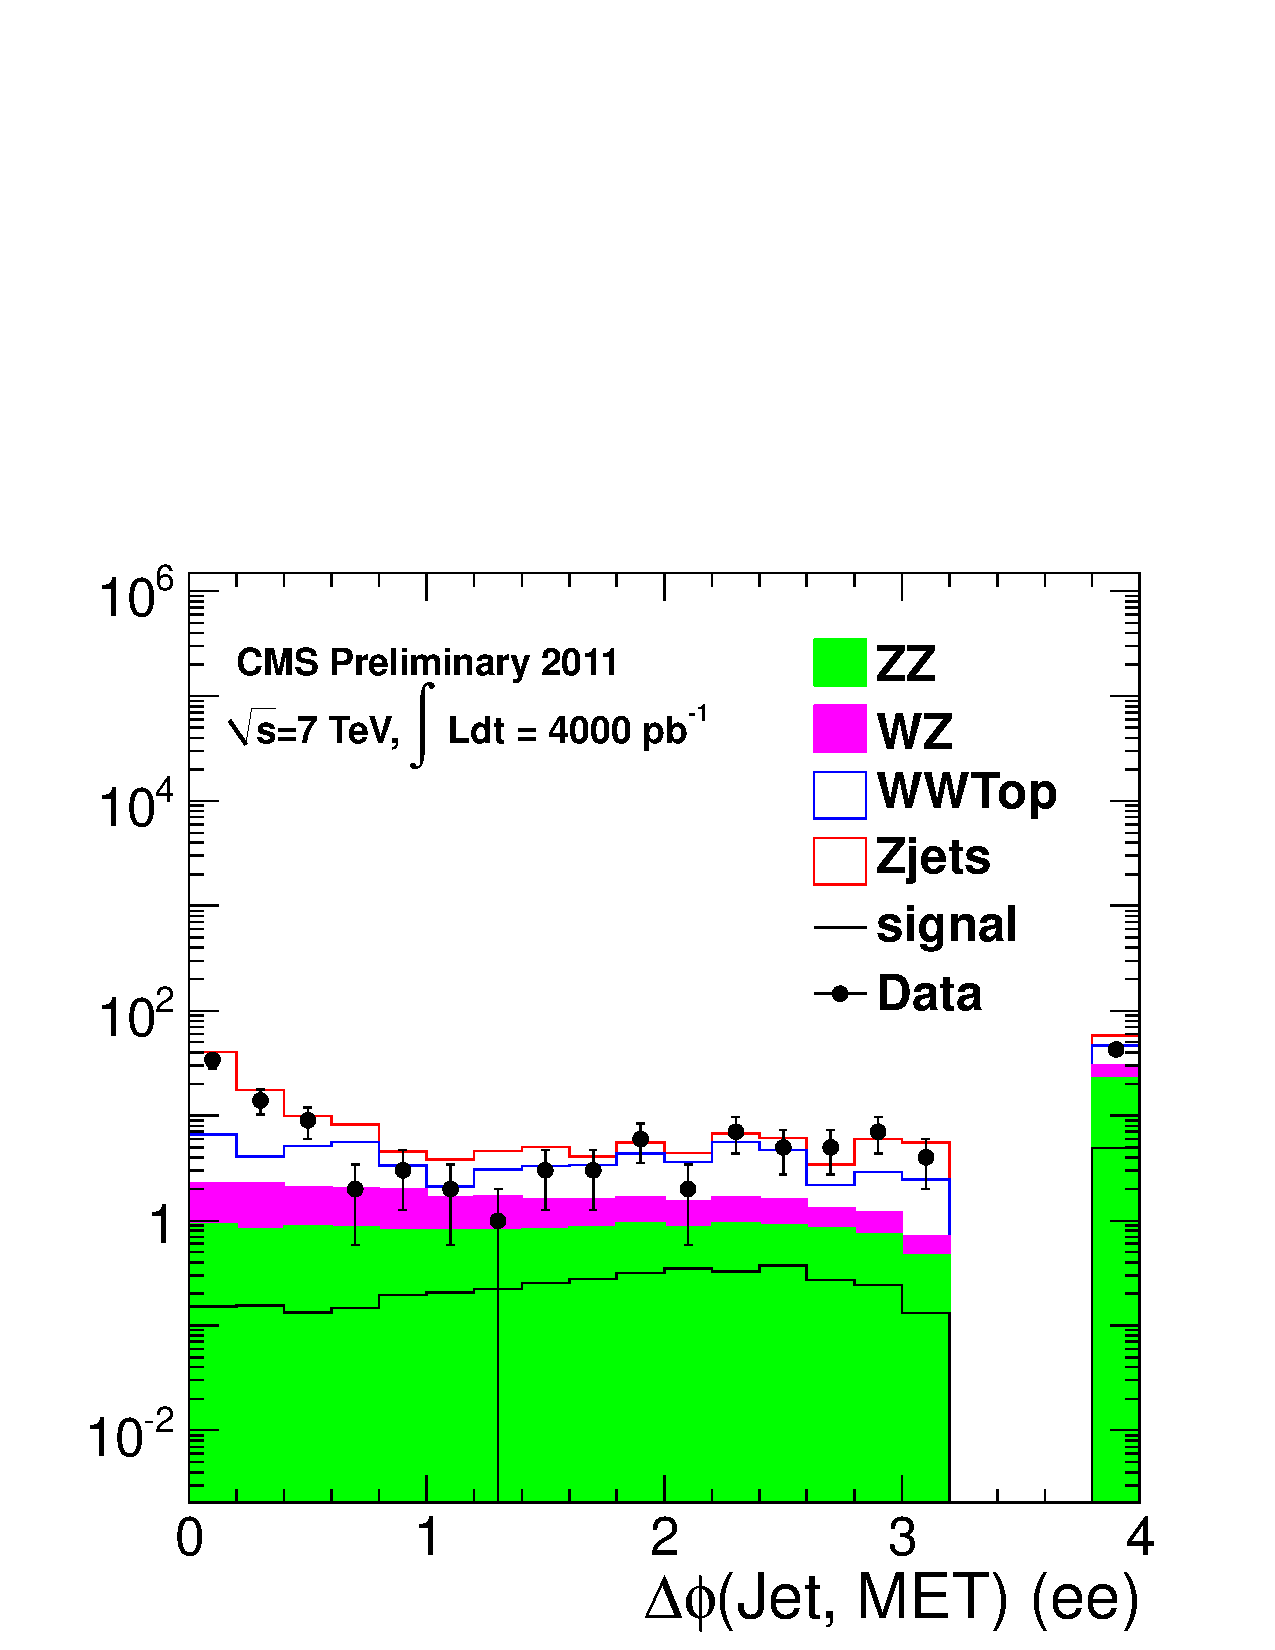
\includegraphics[width=0.4\textwidth]{figures/selection_dphijetmet_ee.pdf}}
\subfigure[$\mu\mu$]{\label{subfig:dphijetmet_mm}
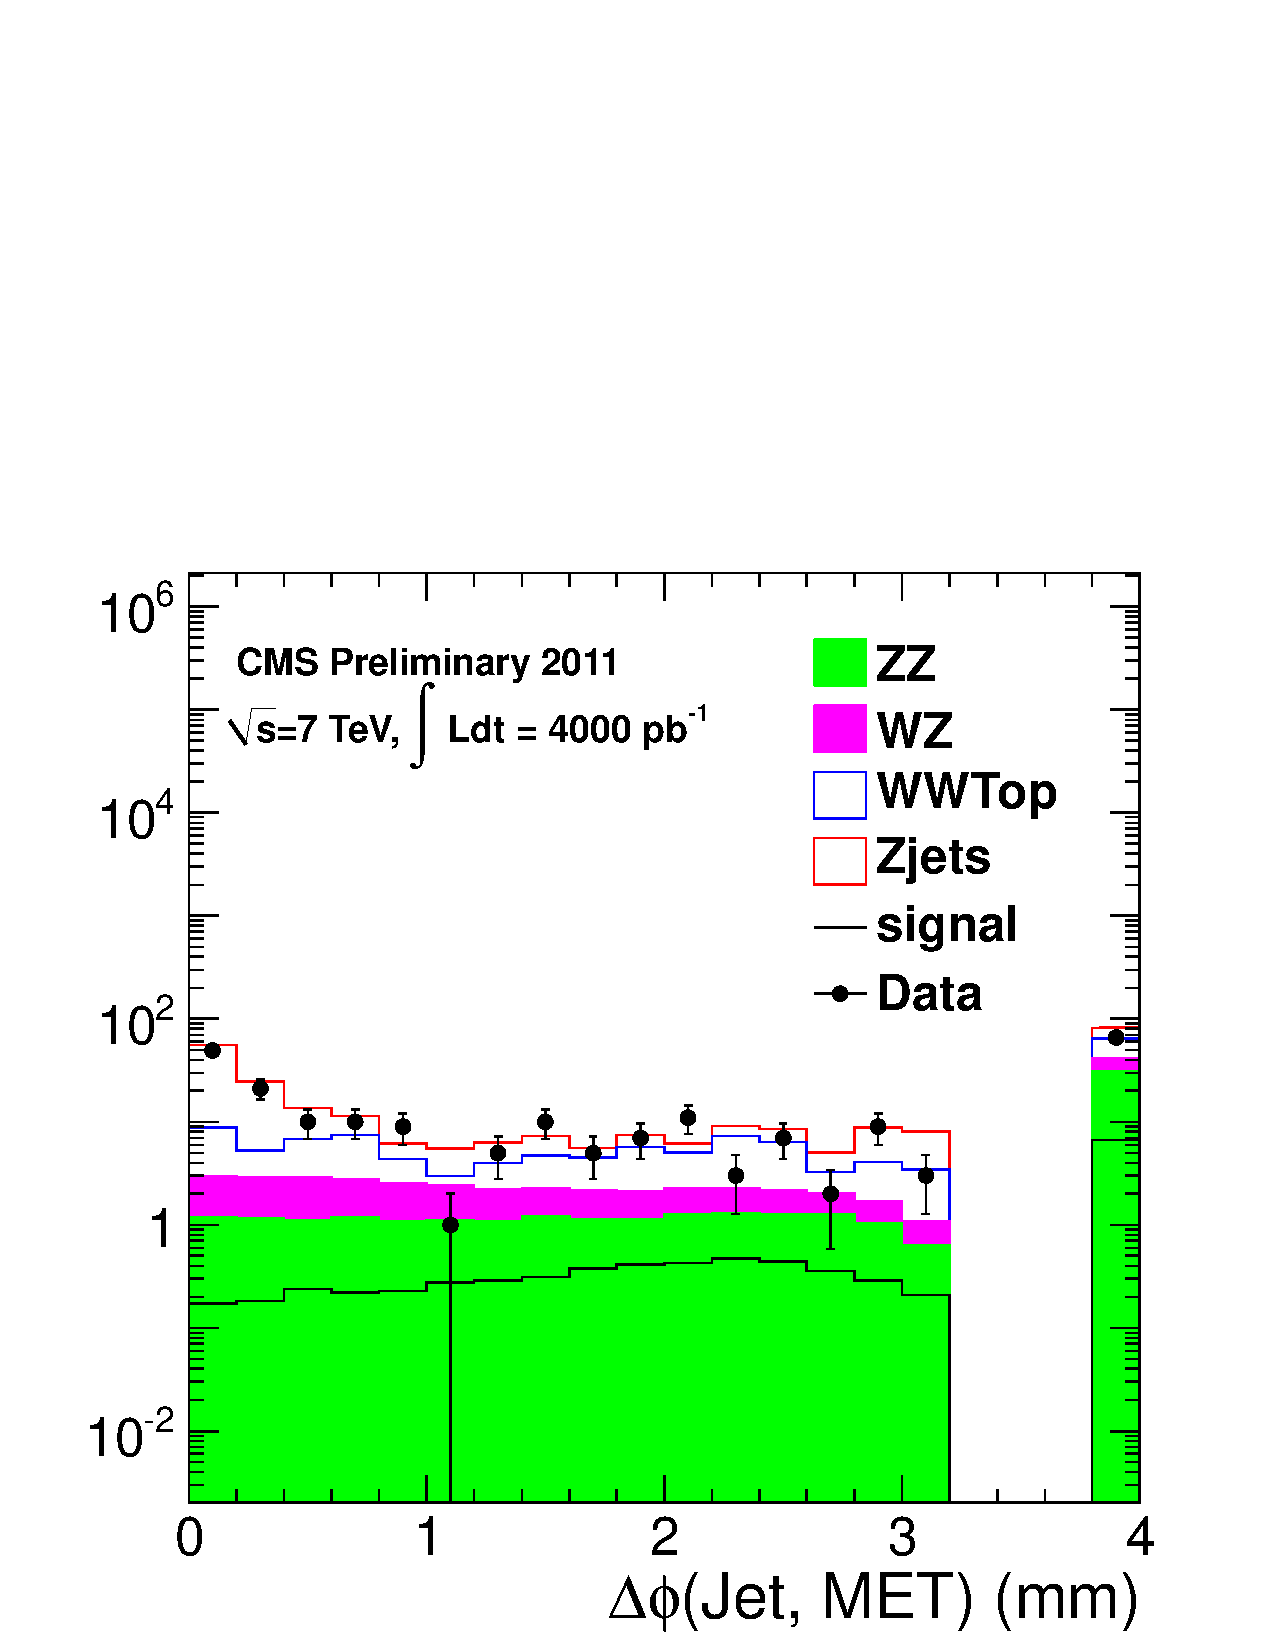
\includegraphics[width=0.4\textwidth]{figures/selection_dphijetmet_mm.pdf}}
\caption{The $\Delta\phi(jet,\met)$ between the \met\, and the nearest jet (with $\Et>30\,\GeV$) 
in the $ee$ (left) and $\mu\mu$ (right) channels. 
The overflow bin represents those events with zero jets.}
\label{fig:mtemloosesel}
\end{center}
\end{figure}
%%%%%%%%%%%%%%%

\begin{table}[!ht]
\begin{center}
\begin{tabular}{c|cccccc}\hline
Mass & 250 & 300 & 350 & 400 & 500 & 600 \\ \hline 
Met & $>   70$ & $>   79$ & $>   95$ & $>  115$ & $>  150$ & $>  161$ \\ 
 $M_T$ & [$ 222$,~$ 272$] & [$ 264$,~$ 331$] & [$ 298$,~$ 393$] & [$ 327$,~$ 460$] & [$ 382$,~$ 605$] & [$ 452$,~$ 767$] \\ 
 $\Delta\phi(\mathrm{Jet}, \mathrm{MET})$ & $> 0.47$ & $> 0.33$ & $> 0.21$ & $> 0.12$ & $> 0.01$ & $> 0.00$ \\ \hline
 \end{tabular}
\caption{Table of cuts as a function of Higgs boson mass in the cut-based analysis.}
\label{tab:cut_selection}
\end{center}
\end{table}

